% Provenance (never printed): see sources/outline_sources.md (Year 2: humidity variables;
% Clausius--Clapeyron applied; dry and moist adiabats; thermodynamic diagrams; convective
% instability; cloud microphysics). Definitions after the NWS glossary; skew-T lines, CAPE classes
% and the lifted index after the NWS Houston/Galveston training page; saturation data from the
% NIST WebBook (IAPWS-95) and IAPWS R14-08; the empirical formula as used by Su and others
% (2026); kappa-Koehler theory after Petters and Kreidenweis (2007); CCN numbers after Andreae
% (2009); the processes of microphysics after Morrison and others (2020). The sounding is the
% real 12 UTC sounding of Norman, Oklahoma, 16 April 2026 (IGRA2); every curve and number from
% figdata/bachelor-2/thermo.py; exercise and problem values in the Book 4 scratch calculator
% calc/ch21.py.
\chapter{Atmospheric Thermodynamics}\label{ch:b2:atmospheric-thermodynamics}

On 16 April 2026, at 12 UTC, a balloon rose from the weather station of Norman, Oklahoma, as
balloons rise from more than eight hundred stations at that hour every day. The instrument it
carried radioed back a vertical profile that a forecaster reads at a glance: air near the ground
almost saturated, a thin warm lid six hundred metres up, and above it a temperature falling
fast for ten kilometres. Lifted through the lid, the surface air would have found itself
warmer than its surroundings over most of the troposphere, with some two thousand joules per
kilogram to spend on rising. This chapter learns to read that energy from a sounding: how much
water air holds, how a rising parcel cools before and after it condenses, how the diagrams of
meteorologists turn areas into energies, and how cloud droplets form at all.
% ledger: data:b4-sounding, nws4:upperair, nws4:cape

\begin{recall}
\textbf{From the physics books}: saturation \omterm{def:b2:atmospheric-thermodynamics:moist-air}{vapour pressure}, relative humidity, dew point,
latent heat, the Clausius--Clapeyron relation and its integrated form; nucleation and
supercooling; the first law, adiabatic changes and the heat capacities of an ideal gas.
\textbf{From the chemistry books}: partial pressures, Raoult's law, surface tension and the Kelvin
equation. \textbf{From the school volumes}: the \omterm{def:b2:atmospheric-thermodynamics:lcl}{condensation level} and its rule of
\qty{125}{m} per degree, stable and unstable air, the \omterm{def:b2:atmospheric-thermodynamics:microphysics}{condensation nucleus}, the warm-rain and
ice-crystal processes. \textbf{From the Year 1 volume}: the standard atmosphere, the environmental
and dry adiabatic lapse rates ($\Gamma_d = \qty{9.8}{K/km}$), the air parcel, the potential
temperature, static stability, temperature inversions and the hypsometric equation.
\end{recall}

Throughout the chapter: $R_d = R/M_d = \qty{287.0}{J.kg^{-1}.K^{-1}}$ for dry air of molar mass
\qty{28.97}{g/mol}; $R_v = R/M_w = \qty{461.5}{J.kg^{-1}.K^{-1}}$ for water vapour, of molar
mass \qty{18.0153}{g/mol}; $\varepsilon = M_w/M_d = 0.622$; $c_p = \tfrac72 R_d =
\qty{1004.5}{J.kg^{-1}.K^{-1}}$ (the Year 1 volume, with the ratio of heat capacities 1.4);
$g = \qty{9.81}{m.s^{-2}}$; and the latent heat of vaporization at the triple point,
$L = \qty{2.501e6}{J/kg}$.
% ledger: const:R, earth:Mmol, nist4:water-mw, nasa:grc-gamma, const:gn, nist4:water-sat

\section{Moist air}\label{sec:b2:atmospheric-thermodynamics:moist-air}

Air is a mixture of dry air and water vapour, both close to ideal gases. The physics books
measure its water by the relative humidity and the dew point; a rising parcel needs measures
that do not change when it expands.

\begin{definition}[Vapour pressure; mixing ratio; specific humidity]\label{def:b2:atmospheric-thermodynamics:moist-air}
The \emph{vapour pressure}\index{vapour pressure} $e$ of moist air is the partial pressure of
its water vapour. Its \emph{mixing ratio}\index{mixing ratio} is $r = m_v/m_d$, the mass of water
vapour per unit mass of dry air in the same volume, and its \emph{specific
humidity}\index{specific humidity} is $q = m_v/(m_d + m_v)$, the mass of vapour per unit mass of
moist air. Both are usually given in grams per kilogram.
\end{definition}
% ledger: nws4:humidity

\begin{proposition}[Humidity variables]\label{prop:b2:atmospheric-thermodynamics:humidity}
In moist air at the total pressure $p$ with the \omterm{def:b2:atmospheric-thermodynamics:moist-air}{vapour pressure} $e$,
\[
  r = \frac{\varepsilon e}{p - e}, \qquad q = \frac{r}{1 + r} = \frac{\varepsilon e}{p - (1 -
  \varepsilon)e} .
\]
At saturation, $e = e_s(T)$ and $r = r_s(T, p)$, the saturation \omterm{def:b2:atmospheric-thermodynamics:moist-air}{mixing ratio}. Neither $r$ nor
$q$ changes when a parcel expands or is compressed without gaining or losing water.
\end{proposition}

\begin{proof}
In the same volume $V$ at the temperature $T$, each gas obeys its own ideal-gas law with its
partial pressure: $m_v = eV/(R_vT)$ and $m_d = (p - e)V/(R_dT)$, so $r = (R_d/R_v)\,e/(p - e)$,
and $R_d/R_v = M_w/M_d = \varepsilon$. Dividing $m_v$ by $m_d + m_v$ gives $q = r/(1 + r)$.
Expansion changes $V$, $p$ and $e$ but not the two masses.
\end{proof}

\begin{definition}[Virtual temperature]\label{def:b2:atmospheric-thermodynamics:virtual}
The \emph{virtual temperature}\index{virtual temperature} $T_v$ of moist air is the temperature
that dry air would need, at the same pressure, to have the same density:
\[
  T_v = T\,\frac{1 + r/\varepsilon}{1 + r} \approx T\,(1 + 0.61\,r) .
\]
\end{definition}
% ledger: nws4:virtual-theta-e

The proof that this temperature does what it says is a line: the density of moist air is
$(m_d + m_v)/V = \bigl(p - e\bigr)/(R_dT) + e/(R_vT)$, which, with $e = pr/(\varepsilon + r)$,
equals $p/(R_dT_v)$. Water vapour is lighter than dry air, so moist air is less dense than dry
air at the same temperature and pressure, as if it were a little warmer.

\begin{example}[The air at Norman]\label{ex:b2:atmospheric-thermodynamics:norman}
At the ground the sounding gives $p = \qty{971.1}{hPa}$, $T = \qty{19.0}{\celsius}$ and a dew
point of \qty{18.5}{\celsius}. The \omterm{def:b2:atmospheric-thermodynamics:moist-air}{vapour pressure} is the saturation \omterm{def:b2:atmospheric-thermodynamics:moist-air}{vapour pressure} at the dew
point, $e = e_s(\qty{18.5}{\celsius}) = \qty{21.5}{hPa}$ (\cref{prop:b2:atmospheric-thermodynamics:es}
below). Then $r = 0.622 \times 21.5/(971.1 - 21.5) = \qty{14.1}{g/kg}$, $q = \qty{13.9}{g/kg}$,
and $T_v - T = 0.61 \times 0.0141 \times \qty{292.15}{K} = \qty{2.5}{K}$: this air is as light as
dry air two and a half degrees warmer.
\end{example}
% ledger: data:b4-sounding

\section{Saturation vapour pressure}\label{sec:b2:atmospheric-thermodynamics:saturation}

Over a flat surface of pure water, the \omterm{def:b2:atmospheric-thermodynamics:moist-air}{vapour pressure} at equilibrium depends only on the
temperature. The physics books derive its law, the Clausius--Clapeyron relation, and integrate it
with a constant latent heat; for water vapour, $M L/R = L/R_v$.

\begin{proposition}[Saturation vapour pressure]\label{prop:b2:atmospheric-thermodynamics:es}
With the latent heat $L$ held constant, the saturation \omterm{def:b2:atmospheric-thermodynamics:moist-air}{vapour pressure} over water is
\[
  e_s(T) = e_t \exp\!\Bigl[\frac{L}{R_v}\Bigl(\frac{1}{T_t} - \frac{1}{T}\Bigr)\Bigr],
  \qquad e_t = \qty{6.117}{hPa}, \quad T_t = \qty{273.16}{K}, \quad \frac{L}{R_v} =
  \qty{5419}{K},
\]
where $(T_t, e_t)$ is the triple point of water.
\end{proposition}
% ledger: iapws4:sublimation, nist4:water-sat

\begin{corollary}[Seven per cent per kelvin]\label{cor:b2:atmospheric-thermodynamics:seven}
The relative rate of increase of the saturation \omterm{def:b2:atmospheric-thermodynamics:moist-air}{vapour pressure} is
$\mathrm{d}\ln e_s/\mathrm{d}T = L/(R_v T^2)$: \qty{7.3}{\percent} per kelvin at
\qty{0}{\celsius}, \qty{6.3}{\percent} at \qty{20}{\celsius}, \qty{5.9}{\percent} at
\qty{30}{\celsius}.
\end{corollary}

The constant latent heat is the formula's only flaw: the latent heat falls from
\qty{2500.9}{kJ/kg} at the triple point to \qty{2453.5}{kJ/kg} at \qty{20}{\celsius}, so the
formula runs ahead of the measured values as the temperature rises, by \qty{1.2}{\percent} at
\qty{20}{\celsius} and \qty{2.5}{\percent} at \qty{30}{\celsius} (figure below). An empirical
formula fitted to measurements, $e_s = \qty{6.112}{hPa} \times \exp[17.67\,t/(t + 243.5)]$ with
$t$ in degrees Celsius, stays within a few parts in a thousand; data products use it, but the
proposition is the one that can be differentiated and understood, and this chapter keeps it.
% ledger: nist4:water-sat, su26:svp

Below \qty{0}{\celsius}, water can stay liquid in clouds, supercooled, and two saturation
\omterm{def:b2:atmospheric-thermodynamics:moist-air}{vapour pressures} exist: over liquid water and over ice. The second is lower, because the latent
heat of sublimation exceeds that of vaporization by the latent heat of fusion. Air saturated with
respect to supercooled droplets is supersaturated with respect to ice, by \qty{10}{\percent} at
\qty{-10}{\celsius} and \qty{22}{\percent} at \qty{-20}{\celsius}: the last section returns to
that difference.
% ledger: iapws4:sublimation, su26:svp

\begin{omfigure}
\centering
% figdata/bachelor-2/thermo.py parts es, nist
\begin{tikzpicture}
\begin{groupplot}[group style={group size=2 by 1, horizontal sep=1.9cm},
  width=0.44\linewidth, height=5.4cm, tick label style={font=\scriptsize},
  label style={font=\small}]
\nextgroupplot[xmin=-40, xmax=40, ymin=0, ymax=80, xlabel={temperature (\unit{\celsius})},
  ylabel={saturation vapour pressure (\unit{hPa})}, legend pos=north west,
  legend style={font=\scriptsize, draw=none, fill=none}, legend cell align=left]
\addplot[ocBlue, thick] table[x=T_C, y=cc] {figdata/out/bachelor-2-thermo-es.dat};
\addlegendentry{proposition}
\addplot[black, densely dashed] table[x=T_C, y=emp] {figdata/out/bachelor-2-thermo-es.dat};
\addlegendentry{empirical formula}
\addplot[only marks, mark=*, mark size=1.4pt, ocRed] table[x=T_C, y=es_hPa]
  {figdata/out/bachelor-2-thermo-nist.dat};
\addlegendentry{measured (IAPWS-95)}
\nextgroupplot[xmin=-40, xmax=0, ymin=1, ymax=1.5, xlabel={temperature (\unit{\celsius})},
  ylabel={$e_s(\text{water})/e_s(\text{ice})$}]
\addplot[omMeth, thick, unbounded coords=discard] table[x=T_C, y=wi]
  {figdata/out/bachelor-2-thermo-es.dat};
\draw[black!40, densely dotted] (axis cs:-10,1) -- (axis cs:-10,1.1035) -- (axis cs:-40,1.1035);
\node[font=\scriptsize, anchor=south west] at (axis cs:-10,1.1035) {1.10};
\draw[black!40, densely dotted] (axis cs:-20,1) -- (axis cs:-20,1.218) -- (axis cs:-40,1.218);
\node[font=\scriptsize, anchor=south west] at (axis cs:-20,1.218) {1.22};
\end{groupplot}
\end{tikzpicture}
\par\smallskip{\small Left: the saturation \omterm{def:b2:atmospheric-thermodynamics:moist-air}{vapour pressure} over water by
\cref{prop:b2:atmospheric-thermodynamics:es}, by the empirical formula and as measured. Right: the
ratio of the saturation \omterm{def:b2:atmospheric-thermodynamics:moist-air}{vapour pressures} over supercooled water (empirical formula) and over ice
(IAPWS sublimation equation).}
\end{omfigure}
% ledger: nist4:water-sat, iapws4:sublimation, su26:svp

\section{Rising moist air}\label{sec:b2:atmospheric-thermodynamics:ascent}

A parcel that rises without exchanging heat cools at the dry adiabatic lapse rate, keeps its
potential temperature, and, if it does not condense, keeps its \omterm{def:b2:atmospheric-thermodynamics:moist-air}{mixing ratio}. Its \omterm{def:b2:atmospheric-thermodynamics:moist-air}{vapour pressure}
$e = pr/(\varepsilon + r)$ falls with the pressure, but its saturation \omterm{def:b2:atmospheric-thermodynamics:moist-air}{vapour pressure} falls
faster, with its temperature. The two meet at a level that the school volumes found by a rule.

\begin{definition}[Lifting condensation level]\label{def:b2:atmospheric-thermodynamics:lcl}
The \emph{lifting condensation level}\index{lifting condensation level} (LCL) of a parcel is the
level at which it becomes saturated when it is lifted dry adiabatically. It is the
\emph{condensation level}\index{condensation level} of the school volumes, the height of the
flat bases of the clouds that form by lifting.
\end{definition}
% ledger: nws4:lcl

\begin{proposition}[Height of the lifting condensation level]\label{prop:b2:atmospheric-thermodynamics:lcl}
A parcel at the temperature $T$ with the dew point $T_d$ reaches saturation about
\[
  z_{\text{LCL}} \approx \frac{T - T_d}{\Gamma_d - \Gamma_{\text{dew}}}, \qquad
  \Gamma_{\text{dew}} = \frac{g R_v T_d^2}{L R_d T} \approx \qty{1.8}{K/km},
\]
above its starting level: about \qty{125}{m} for each degree of dew-point depression.
\end{proposition}

\begin{proof}
The parcel's temperature falls at $\Gamma_d$. Its dew point is the temperature at which its
\omterm{def:b2:atmospheric-thermodynamics:moist-air}{vapour pressure} $e$ would saturate; with $r$ constant, $e$ is proportional to $p$, so
$\mathrm{d}\ln e = \mathrm{d}\ln p = -g\,\mathrm{d}z/(R_dT)$ by the hydrostatic balance. By
\cref{prop:b2:atmospheric-thermodynamics:es}, $\mathrm{d}\ln e = L\,\mathrm{d}T_d/(R_vT_d^2)$.
Hence $\mathrm{d}T_d/\mathrm{d}z = -gR_vT_d^2/(LR_dT) = -\Gamma_{\text{dew}}$: the dew point falls
too, but more slowly. The gap $T - T_d$ closes at the rate $\Gamma_d - \Gamma_{\text{dew}}$. With
$T \approx T_d \approx \qty{288}{K}$, $\Gamma_{\text{dew}} = \qty{1.8}{K/km}$, and $1/(9.8 - 1.8)$
kilometres per kelvin is \qty{125}{m}.
\end{proof}

At Norman the dew-point depression was \qty{0.5}{K}: the surface air would have condensed after
\qty{63}{m} of ascent, at \qty{964}{hPa}. The full computation, which follows the dry adiabat and
the saturation \omterm{def:b2:atmospheric-thermodynamics:moist-air}{mixing ratio} without linearizing, gives \qty{64}{m}.
% ledger: data:b4-sounding

Above the LCL the parcel condenses as it rises. Condensation releases latent heat, and the parcel
cools more slowly.

\begin{definition}[Saturated adiabatic lapse rate; moist adiabat]\label{def:b2:atmospheric-thermodynamics:moist-adiabat}
The \emph{saturated adiabatic lapse rate}\index{saturated adiabatic lapse rate} $\Gamma_s$ is
the rate at which the temperature of a saturated parcel falls as it rises, its vapour condensing
to keep it saturated. The curve it follows on a diagram of temperature against pressure is a
\emph{moist adiabat}\index{moist adiabat}. When the condensed water is assumed to fall out at
once, the ascent is called pseudo-adiabatic.
\end{definition}
% ledger: nws4:malr

\begin{proposition}[Saturated adiabatic lapse rate]\label{prop:b2:atmospheric-thermodynamics:gamma-s}
For a pseudo-adiabatic ascent, with $r_s = r_s(T, p)$,
\[
  \Gamma_s = g\,\frac{1 + \dfrac{L r_s}{R_d T}}{c_p + \dfrac{L^2 r_s}{R_v T^2}} .
\]
It tends to $\Gamma_d = g/c_p$ when $r_s$ tends to zero, and is smaller otherwise.
\end{proposition}

\begin{proof}
Per unit mass of dry air, the first law for a parcel that receives the latent heat of the vapour
it condenses, $-L\,\mathrm{d}r_s$, reads $c_p\,\mathrm{d}T - (R_dT/p)\,\mathrm{d}p = -L\,
\mathrm{d}r_s$; with the hydrostatic balance $(R_dT/p)\,\mathrm{d}p = -g\,\mathrm{d}z$, it becomes
$c_p\,\mathrm{d}T + g\,\mathrm{d}z + L\,\mathrm{d}r_s = 0$. With $r_s \approx \varepsilon e_s/p$,
$\mathrm{d}r_s = r_s\,(\mathrm{d}\ln e_s - \mathrm{d}\ln p) = r_s\bigl(L\,\mathrm{d}T/(R_vT^2) +
g\,\mathrm{d}z/(R_dT)\bigr)$. Substituting and collecting the terms in $\mathrm{d}T$ and in
$\mathrm{d}z$ gives $-\mathrm{d}T/\mathrm{d}z = \Gamma_s$.
\end{proof}

The rate depends on how much water there is to condense. At \qty{1000}{hPa} it is
\qty{6.5}{K/km} at \qty{0}{\celsius}, \qty{5.2}{K/km} at \qty{10}{\celsius}, \qty{4.2}{K/km} at
\qty{20}{\celsius} and \qty{3.4}{K/km} at \qty{30}{\celsius}; high in the troposphere, at
\qty{200}{hPa} and \qty{-60}{\celsius}, it is back to \qty{9.6}{K/km}, almost the dry rate. A
\omterm{def:b2:atmospheric-thermodynamics:moist-adiabat}{moist adiabat} is therefore steep near warm ground and bends towards the dry adiabats aloft.
% ledger: nws4:malr

\begin{definition}[Equivalent potential temperature]\label{def:b2:atmospheric-thermodynamics:theta-e}
The \emph{equivalent potential temperature}\index{equivalent potential temperature} $\theta_e$ of
a parcel is the temperature it would have if it were lifted until all its vapour had condensed
and fallen out, then brought down dry adiabatically to \qty{1000}{hPa}. A good approximation is
\[
  \theta_e \approx \theta \exp\!\Bigl(\frac{L r}{c_p T_{\text{LCL}}}\Bigr),
\]
with $\theta$ the potential temperature and $T_{\text{LCL}}$ the temperature at the parcel's
\omterm{def:b2:atmospheric-thermodynamics:lcl}{lifting condensation level}.
\end{definition}
% ledger: nws4:virtual-theta-e

The potential temperature is conserved in dry ascent only; $\theta_e$ is conserved, to this
approximation, in dry and saturated ascent alike, because the heat it counts as already released
is exactly the heat condensation releases. It labels a \omterm{def:b2:atmospheric-thermodynamics:moist-adiabat}{moist adiabat} as $\theta$ labels a dry one.
The Norman surface air has $\theta = 292.15 \times (1000/971.1)^{2/7} = \qty{294.6}{K}$ and
$\theta_e = 294.6 \exp[2.501 \times 10^6 \times 0.0141/(1004.5 \times 291.5)] = \qty{332}{K}$.
% ledger: data:b4-sounding

\section{Thermodynamic diagrams}\label{sec:b2:atmospheric-thermodynamics:diagrams}

\begin{definition}[Atmospheric sounding]\label{def:b2:atmospheric-thermodynamics:sounding}
An \emph{atmospheric sounding}\index{atmospheric sounding} is a vertical profile of the
pressure, temperature, humidity and wind of the atmosphere above a place, measured by an
instrument carried aloft, usually a radiosonde under a balloon.
\end{definition}
% ledger: nws:radiosonde, nws4:upperair

A sounding is not quite vertical, because the balloon drifts with the wind, nor quite
instantaneous, because it takes several minutes to reach the upper troposphere; and the main
network launches only twice a day. Its numbers become useful once they are drawn on a chart
where a rising parcel can be followed with a ruler.
% ledger: hgx:skewt-lines

\begin{definition}[Thermodynamic diagram; skew-T log-p diagram; tephigram]\label{def:b2:atmospheric-thermodynamics:diagram}
A \emph{thermodynamic diagram}\index{thermodynamic diagram} is a chart whose coordinates are
functions of the pressure and the temperature, on which isobars, isotherms, dry adiabats, \omterm{def:b2:atmospheric-thermodynamics:moist-adiabat}{moist
adiabats} and lines of constant saturation \omterm{def:b2:atmospheric-thermodynamics:moist-air}{mixing ratio} are printed, and on which a sounding is
plotted as two curves, its temperature and its dew point. On a \emph{skew-T log-p
diagram}\index{skew-T log-p diagram} the vertical coordinate is $-\ln p$ and the horizontal one is
$T + k\ln(p_0/p)$, so that isobars are horizontal and isotherms are straight lines slanting up to
the right. A \emph{tephigram}\index{tephigram} uses the temperature and the entropy per unit
mass $c_p\ln\theta$ as coordinates, so that isotherms and dry adiabats are perpendicular straight
lines.
\end{definition}
% ledger: hgx:skewt-lines

\begin{proposition}[Areas are energies]\label{prop:b2:atmospheric-thermodynamics:areas}
On a \omterm{def:b2:atmospheric-thermodynamics:diagram}{skew-T log-p diagram}, the area enclosed between two curves $T_1(p)$ and $T_2(p)$ over the
pressures $p_b > p_a$ is proportional to $\int_{p_a}^{p_b} R_d\,(T_1 - T_2)\,\mathrm{d}\ln p$,
the energy per unit mass that \cref{prop:b2:atmospheric-thermodynamics:buoyancy} below gives to
a parcel following $T_1$ through an environment $T_2$.
\end{proposition}

\begin{proof}
Take $Y = \ln(p_0/p)$ and $X = T + kY$. The Jacobian of $(T, Y) \mapsto (X, Y)$ is 1, so areas in
the $(X, Y)$ plane equal areas in the $(T, Y)$ plane, where the area between two curves is
$\int (T_1 - T_2)\,\mathrm{d}Y = \int (T_1 - T_2)\,\mathrm{d}\ln p$ taken from $p_a$ to $p_b$
with the sign fixed. Multiplying by $R_d$ and by the scale of the chart gives the energy.
\end{proof}

\begin{method}[Lifting a parcel on a diagram]\label{met:b2:atmospheric-thermodynamics:lift}
\begin{enumerate}
  \item Plot the sounding's temperature and dew point against pressure.
  \item From the parcel's temperature, follow the dry adiabat upward; from its dew point, follow
        the line of saturation \omterm{def:b2:atmospheric-thermodynamics:moist-air}{mixing ratio}. Where they meet is the LCL.
  \item From the LCL, follow the \omterm{def:b2:atmospheric-thermodynamics:moist-adiabat}{moist adiabat} upward.
  \item Where the parcel's curve lies to the right of the sounding's temperature, the parcel is
        warmer than its surroundings; the levels where the two curves cross are the levels of
        \cref{def:b2:atmospheric-thermodynamics:parcel-levels} below.
\end{enumerate}
\end{method}
% ledger: hgx:skewt-lines


\section{Stability and convective energy}\label{sec:b2:atmospheric-thermodynamics:stability}

The Year 1 volume compared the lapse rate $\Gamma$ of a layer with $\Gamma_d$. A saturated
parcel cools at $\Gamma_s$ instead, and a third case appears between the two rates.

\begin{definition}[Conditional instability]\label{def:b2:atmospheric-thermodynamics:instability}
A layer whose lapse rate lies between the saturated and the dry adiabatic lapse rates,
$\Gamma_s < \Gamma < \Gamma_d$, is in \emph{conditional instability}\index{conditional
instability}: stable for unsaturated parcels, unstable for saturated ones.
\end{definition}
% ledger: nws4:malr

At Norman the temperature fell by \qty{37.0}{K} between \qty{850}{hPa} (\qty{1489}{m}) and
\qty{500}{hPa} (\qty{5725}{m}), at \qty{8.7}{K/km}: \omterm{def:b2:atmospheric-thermodynamics:instability}{conditional instability} over four kilometres.
Whether the instability is released depends on where a parcel from below becomes saturated and
then warmer than its surroundings.
% ledger: data:b4-sounding

\begin{definition}[Level of free convection; equilibrium level]\label{def:b2:atmospheric-thermodynamics:parcel-levels}
The \emph{level of free convection}\index{level of free convection} (LFC) of a lifted parcel is
the level above which, saturated, it becomes warmer than its surroundings and rises freely. The
\emph{equilibrium level}\index{equilibrium level} (EL) is the level above the LFC where its
temperature again equals that of its surroundings.
\end{definition}
% ledger: nws4:lfc-el

\begin{omfigure}
\centering
% figdata/bachelor-2/thermo.py parts iso, dry, moist, mix, env, dew, parcel, cape, cin, marks
\begin{tikzpicture}
\begin{axis}[width=0.86\linewidth, height=10.6cm, ymode=log, y dir=reverse, ymin=100,
  ymax=1050, xmin=-42, xmax=44, clip=true,
  ytick={100,200,300,400,500,700,850,1000}, yticklabels={100,200,300,400,500,700,850,1000},
  minor ytick={}, xtick={-41.464,-31.464,-21.464,-11.464,-1.464,8.536,18.536,28.536,38.536},
  xticklabels={$-40$,$-30$,$-20$,$-10$,0,10,20,30,40}, tick label style={font=\scriptsize},
  xlabel={temperature (\unit{\celsius}), read along the slanting isotherms},
  ylabel={pressure (\unit{hPa})}, label style={font=\small},
  legend style={font=\scriptsize, at={(0.985,0.985)}, anchor=north east, fill=white,
  fill opacity=0.9, text opacity=1, draw=black!30}, legend cell align=left]
\addplot[fill=ocRed, fill opacity=0.28, draw=none, forget plot] table[x=x, y=p]
  {figdata/out/bachelor-2-thermo-cape.dat};
\addplot[fill=ocBlue, fill opacity=0.28, draw=none, forget plot] table[x=x, y=p]
  {figdata/out/bachelor-2-thermo-cin.dat};
\addplot[black!22, very thin, forget plot] table[x=x, y=p] {figdata/out/bachelor-2-thermo-iso.dat};
\addplot[orange!70!black, very thin, opacity=0.55] table[x=x, y=p]
  {figdata/out/bachelor-2-thermo-dry.dat};
\addlegendentry{dry adiabats}
\addplot[omMeth, very thin, densely dashed, opacity=0.7] table[x=x, y=p]
  {figdata/out/bachelor-2-thermo-moist.dat};
\addlegendentry{moist adiabats}
\addplot[ocBlue, thin, dotted] table[x=x, y=p]
  {figdata/out/bachelor-2-thermo-mix.dat};
\addlegendentry{saturation mixing ratio}
\addplot[ocRed, thick] table[x=x, y=p] {figdata/out/bachelor-2-thermo-env.dat};
\addlegendentry{temperature}
\addplot[omMeth!70!black, thick] table[x=x, y=p] {figdata/out/bachelor-2-thermo-dew.dat};
\addlegendentry{dew point}
\addplot[black, thick, dashed] table[x=x, y=p] {figdata/out/bachelor-2-thermo-parcel.dat};
\addlegendentry{surface parcel}
\foreach \r/\x in {1/-7.948, 2/0.283, 4/9.053, 8/18.396, 16/28.323} {
  \edef\tmp{\noexpand\node[font=\noexpand\tiny, ocBlue, anchor=south] at (axis cs:\x,600) {\r};}\tmp
}
\addplot[only marks, mark=*, mark size=1.6pt, black, forget plot] table[x=x, y=p]
  {figdata/out/bachelor-2-thermo-marks.dat};
\node[font=\scriptsize, anchor=west] at (axis cs:20.5,963.9) {LCL};
\node[font=\scriptsize, anchor=west] at (axis cs:18.2,732.5) {LFC};
\node[font=\scriptsize, anchor=east] at (axis cs:-9.6,235.6) {EL};
\node[font=\scriptsize, ocRed!70!black] at (axis cs:2,420) {CAPE};
\node[font=\scriptsize, ocBlue!70!black, anchor=west] at (axis cs:27,860) {CIN};
\end{axis}
\end{tikzpicture}
\par\smallskip{\small The 12 UTC sounding of Norman, Oklahoma, on 16 April 2026, on a \omterm{def:b2:atmospheric-thermodynamics:diagram}{skew-T
log-p diagram}, with the surface parcel lifted along its dry adiabat to the LCL and its \omterm{def:b2:atmospheric-thermodynamics:moist-adiabat}{moist
adiabat} above. Red: the positive area (CAPE); blue: the negative area below the LFC (CIN), both
computed with the temperature. Saturation \omterm{def:b2:atmospheric-thermodynamics:moist-air}{mixing ratios} in grams per kilogram, labelled at
\qty{600}{hPa}.}
\end{omfigure}
% ledger: data:b4-sounding, hgx:skewt-lines

\begin{definition}[Convective available potential energy; convective inhibition]\label{def:b2:atmospheric-thermodynamics:cape}
The \emph{convective available potential energy}\index{convective available potential energy}
(CAPE) of a parcel is the work of the buoyancy force on unit mass of it between its LFC and its
EL,
\[
  \text{CAPE} = \int_{z_{\text{LFC}}}^{z_{\text{EL}}} g\,\frac{T_{v,\text{parcel}} -
  T_{v,\text{env}}}{T_{v,\text{env}}}\,\mathrm{d}z ,
\]
and its \emph{convective inhibition}\index{convective inhibition} (CIN) is the same integral,
negative, from its starting level to its LFC.
\end{definition}
% ledger: nws4:cape, nws4:cin

\begin{proposition}[Buoyancy on a diagram; the parcel's speed]\label{prop:b2:atmospheric-thermodynamics:buoyancy}
\begin{enumerate}
  \item In terms of pressure, $\text{CAPE} = R_d \int_{p_{\text{EL}}}^{p_{\text{LFC}}}
        (T_{v,\text{parcel}} - T_{v,\text{env}})\,\mathrm{d}\ln p$: on a \omterm{def:b2:atmospheric-thermodynamics:diagram}{skew-T log-p diagram}, it is
        proportional to the area between the parcel's curve and the sounding.
  \item A parcel that leaves the LFC at rest and keeps all the work of its buoyancy reaches the
        EL with the vertical speed $w_{\max} = \sqrt{2\,\text{CAPE}}$.
\end{enumerate}
\end{proposition}

\begin{proof}
1. The parcel and its surroundings share the pressure, so the density ratio is the ratio of the
\omterm{def:b2:atmospheric-thermodynamics:virtual}{virtual temperatures} and the buoyancy force per unit mass is
$g(T_{v,\text{parcel}} - T_{v,\text{env}})/T_{v,\text{env}}$. The environment is hydrostatic:
$\mathrm{d}z = -R_dT_{v,\text{env}}\,\mathrm{d}\ln p/g$. Substituting cancels $g$ and
$T_{v,\text{env}}$; the area follows from \cref{prop:b2:atmospheric-thermodynamics:areas}.
2. With $b$ the buoyancy force per unit mass, $\mathrm{d}w/\mathrm{d}t = b$ and $w = \mathrm{d}z/
\mathrm{d}t$ give $w\,\mathrm{d}w = b\,\mathrm{d}z$; integrating from the LFC, where $w = 0$, to
the EL gives $w^2/2 = \text{CAPE}$.
\end{proof}

\begin{example}[The energy in the Norman sounding]\label{ex:b2:atmospheric-thermodynamics:cape}
Lift the surface air of \cref{ex:b2:atmospheric-thermodynamics:norman}. It saturates at
\qty{964}{hPa}, \qty{64}{m} up, and follows a \omterm{def:b2:atmospheric-thermodynamics:moist-adiabat}{moist adiabat}. Below \qty{900}{hPa} the sounding is
itself nearly saturated and the parcel stays a few tenths of a degree colder than its
surroundings; then comes the inversion between \qty{908}{hPa} and \qty{889}{hPa}, where the
temperature rises by \qty{4.1}{K} in \qty{178}{m} and the parcel finds itself \qty{5}{K} too
cold. It becomes warmer than its surroundings only at \qty{732}{hPa}, \qty{2.4}{km} above the
ground, its LFC, and stays warmer up to its EL at \qty{236}{hPa}, \qty{10.9}{km} above sea level,
just below the tropopause the sounding reports at \qty{235}{hPa}. On a fine grid of pressures the
areas of the skew-T figure are CAPE $= \qty{2100}{J/kg}$ and CIN $= \qty{-200}{J/kg}$ with the
temperature, and \qty{2230}{J/kg} and \qty{-130}{J/kg} with the \omterm{def:b2:atmospheric-thermodynamics:virtual}{virtual temperature}: the moisture
of the parcel adds its own buoyancy. Parcel theory gives $w_{\max} = \sqrt{2 \times 2100} =
\qty{65}{m/s}$.
\end{example}
% ledger: data:b4-sounding

Forecasters' tables call a CAPE up to \qty{1500}{J/kg} positive, one between 1500 and
\qty{2500}{J/kg} large and one above \qty{2500}{J/kg} extreme; values above \qty{1000}{J/kg} are common in thunderstorm environments,
and rare ones exceed \qty{5000}{J/kg}. CAPE is largest in the warm season, especially in late
spring. The lifted index, the sounding's temperature at \qty{500}{hPa} minus that of the lifted
parcel, sums the same information in one number: at Norman, $-18.4 - (-8.9) = \qty{-9.5}{K}$,
in the class from $-8$ to $-10$ that the forecasters' tables call extreme instability. None of
these values is a threshold above which storms must form.
% ledger: hgx:cape, nws4:cape, nws4:lifted-index

The CIN is the price of admission. The warm lid kept the surface air from rising on its own: a
parcel would have to be pushed through it, by a front or by the slow ascent of the air ahead of
a disturbance aloft, or warmed from below by the afternoon sun until it was buoyant all the way.
And the speed $w_{\max}$ is an upper bound: a real updraft carries its condensed water, which
weighs it down, and mixes with the drier air around it, which cools it by evaporation. The
\omterm{def:b2:atmospheric-thermodynamics:parcel-levels}{equilibrium level} remains a good guide to where the storm tops spread out into an anvil.
% ledger: nws4:cin, hgx:cape, nws4:lfc-el

\begin{omfigure}
\centering
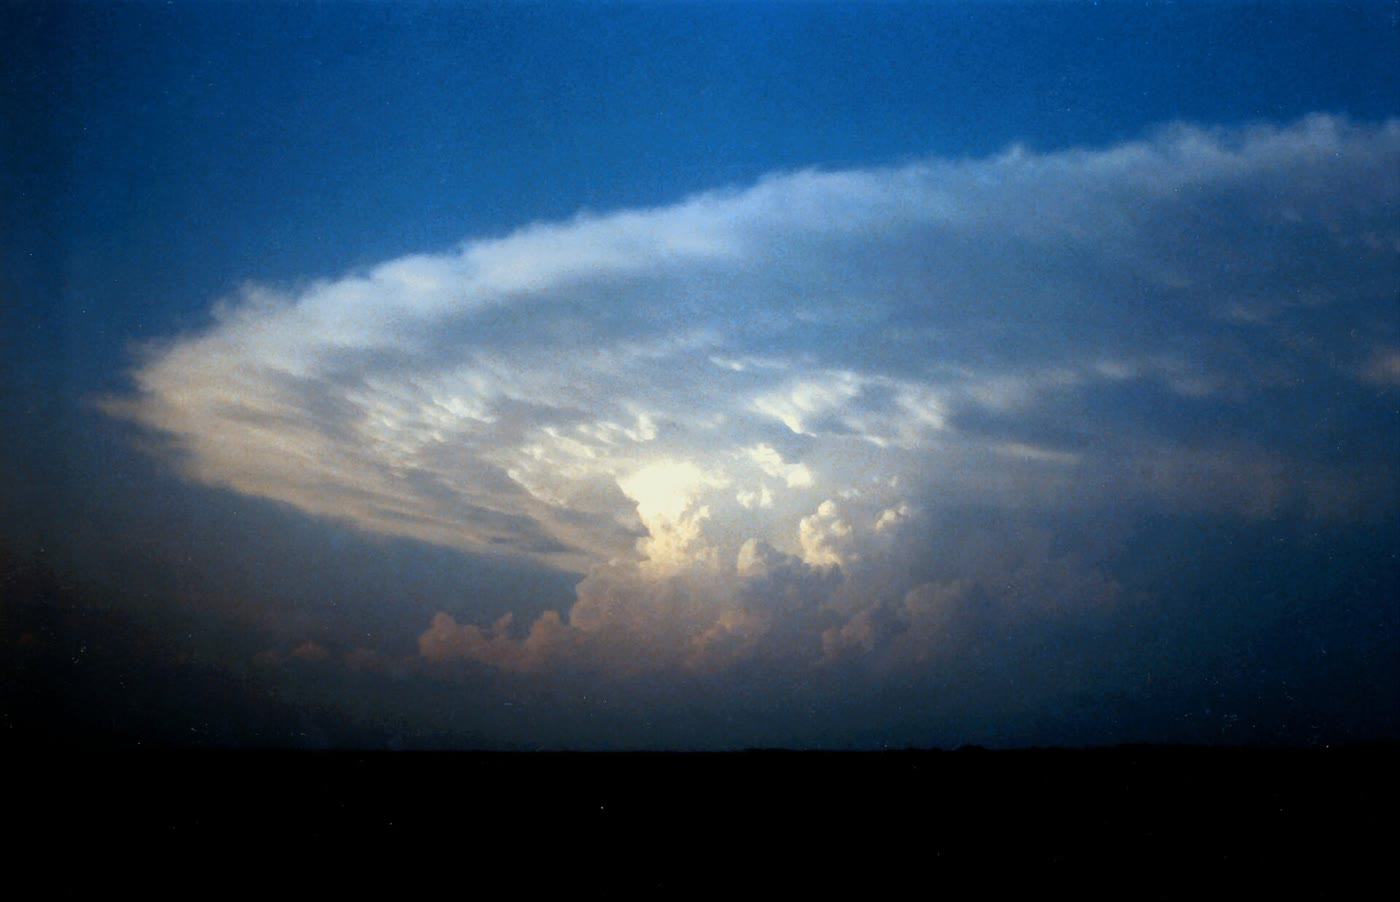
\includegraphics[width=0.6\linewidth]{images/book4/b2-21-supercell-anvil.jpg}
\par\smallskip{\small A thunderstorm over Nebraska, 20 April 1985: its updraft spreads out into
an anvil where it reaches its \omterm{def:b2:atmospheric-thermodynamics:parcel-levels}{equilibrium level}, near the tropopause. (Stephen Corfidi,
NOAA/NWS, public domain, via Wikimedia Commons.)}
\end{omfigure}
% ledger: nws4:lfc-el

\section{Cloud microphysics}\label{sec:b2:atmospheric-thermodynamics:microphysics}

A parcel at its LCL is saturated over a flat water surface. A droplet is not flat: the physics
books show that a new phase does not appear at equilibrium, but only through nucleation, and the
chemistry books that the \omterm{def:b2:atmospheric-thermodynamics:moist-air}{vapour pressure} over a curved surface exceeds that over a flat one
(the Kelvin equation). With the constant $A$ of \cref{prop:b2:atmospheric-thermodynamics:kohler}
below, a droplet of pure water \qty{2}{nm} across is in equilibrium only at the saturation ratio
$\exp(2.1/2) = 2.9$, a \omterm{def:b2:atmospheric-thermodynamics:microphysics}{supersaturation} of \qty{190}{\percent}, far above the fractions of a per
cent at which particles activate: droplets form on particles.

\begin{definition}[Supersaturation; cloud condensation nucleus]\label{def:b2:atmospheric-thermodynamics:microphysics}
The \emph{supersaturation}\index{supersaturation} of air is $s = e/e_s - 1$, the excess of its
\omterm{def:b2:atmospheric-thermodynamics:moist-air}{vapour pressure} over the saturation \omterm{def:b2:atmospheric-thermodynamics:moist-air}{vapour pressure} above a flat surface of pure water, usually
given in per cent. A \emph{cloud condensation nucleus}\index{cloud condensation nucleus} (CCN)
is an aerosol particle on which a cloud droplet forms at the small supersaturations of clouds.
It is the \emph{condensation nucleus}\index{condensation nucleus} of the school volumes.
\end{definition}
% ledger: nws4:ccn-bergeron, pk07:kohler, morrison20:processes

\begin{proposition}[Köhler curve]\label{prop:b2:atmospheric-thermodynamics:kohler}
\index{Köhler curve}
A solution droplet of diameter $D$ grown on a dry particle of diameter $D_d$ and hygroscopicity
$\kappa$ is in equilibrium with the saturation ratio
\[
  S(D) = \frac{D^3 - D_d^3}{D^3 - D_d^3(1 - \kappa)}\,\exp\Bigl(\frac{A}{D}\Bigr), \qquad
  A = \frac{4\sigma M_w}{R T\rho_w},
\]
with $\sigma$ the surface tension and $\rho_w$ the density of water (admitted). The curve $S(D)$
is the \emph{\omterm{prop:b2:atmospheric-thermodynamics:kohler}{Köhler curve}}. For $D \gg D_d$,
\[
  s = S - 1 \approx \frac{A}{D} - \frac{\kappa D_d^3}{D^3},
\]
which is maximal at the critical diameter and \omterm{def:b2:atmospheric-thermodynamics:microphysics}{supersaturation}
\[
  D_c = \sqrt{\frac{3\kappa D_d^3}{A}}, \qquad s_c = \sqrt{\frac{4A^3}{27\,\kappa D_d^3}} .
\]
\end{proposition}
% ledger: pk07:kohler

\begin{proof}[Proof of the approximation]
The exponential is the Kelvin factor; the fraction is the water activity, a version of Raoult's
law in which $\kappa$ measures how much water the dissolved matter binds. For $D \gg D_d$ and
$A \ll D$, $\exp(A/D) \approx 1 + A/D$ and the fraction is $1 - \kappa D_d^3/D^3$ to first
order; the product, to first order, is $1 + A/D - \kappa D_d^3/D^3$. Setting the derivative
$-A/D^2 + 3\kappa D_d^3/D^4$ to zero gives $D_c^2 = 3\kappa D_d^3/A$, and then $s_c = A/D_c -
A/(3D_c) = 2A/(3D_c)$, which is the formula.
\end{proof}

With $\sigma = \qty{0.072}{J/m^2}$ at \qty{298.15}{K}, $A = \qty{2.1}{nm}$. Ammonium sulfate has
$\kappa = 0.61$; sodium chloride is more hygroscopic still ($\kappa = 1.28$), and atmospheric particles mostly lie between 0.1 and 0.9.
A dry particle of \qty{50}{nm} of ammonium sulfate has $D_c = \qty{0.33}{\micro m}$ and $s_c =
\qty{0.42}{\percent}$; one of \qty{100}{nm}, \qty{0.93}{\micro m} and \qty{0.15}{\percent}. The
approximation differs from the exact maximum by less than \qty{1}{\percent}.
% ledger: pk07:kohler, pk07:kappa

\begin{omfigure}
\centering
% figdata/bachelor-2/thermo.py part kohler
\begin{tikzpicture}
\begin{semilogxaxis}[width=0.72\linewidth, height=5.6cm, xmin=0.03, xmax=10, ymin=-0.4,
  ymax=1.1, xlabel={droplet diameter $D$ (\unit{\micro m})}, ylabel={supersaturation $s$
  (\unit{\percent})}, tick label style={font=\scriptsize}, label style={font=\small},
  log ticks with fixed point, legend style={font=\scriptsize, draw=none, fill=none},
  legend pos=north east, legend cell align=left, unbounded coords=discard]
\addplot[ocBlue, thick, densely dotted] table[x=D_um, y=s30] {figdata/out/bachelor-2-thermo-kohler.dat};
\addlegendentry{$D_d = \qty{30}{nm}$}
\addplot[ocBlue, thick] table[x=D_um, y=s50] {figdata/out/bachelor-2-thermo-kohler.dat};
\addlegendentry{$D_d = \qty{50}{nm}$}
\addplot[ocBlue, thick, dashed] table[x=D_um, y=s100] {figdata/out/bachelor-2-thermo-kohler.dat};
\addlegendentry{$D_d = \qty{100}{nm}$}
\addplot[only marks, mark=*, mark size=1.5pt, black] coordinates {(0.1542,0.914) (0.3309,0.4244)
  (0.9345,0.1499)};
\draw[black!45] (axis cs:0.03,0) -- (axis cs:10,0);
\draw[ocRed, densely dashed] (axis cs:0.03,0.5) -- (axis cs:10,0.5);
\node[font=\scriptsize, ocRed, anchor=north west] at (axis cs:2.2,0.5) {$s = \qty{0.5}{\percent}$};
\end{semilogxaxis}
\end{tikzpicture}
\par\smallskip{\small \omterm{prop:b2:atmospheric-thermodynamics:kohler}{Köhler curves} of ammonium sulfate particles ($\kappa = 0.61$) of three dry
diameters at \qty{298.15}{K}, with their critical points (dots). In air at \qty{0.5}{\percent}
\omterm{def:b2:atmospheric-thermodynamics:microphysics}{supersaturation}, the \qty{50}{nm} and \qty{100}{nm} particles grow without limit; the
\qty{30}{nm} particle stays a haze droplet.}
\end{omfigure}
% ledger: pk07:kohler, pk07:kappa

The curve divides the particles. Below its peak a droplet is in stable equilibrium: if it grows,
the air is no longer supersaturated enough for it and it shrinks back; such haze droplets swell
and shrink with the humidity. Once the \omterm{def:b2:atmospheric-thermodynamics:microphysics}{supersaturation} of the air exceeds $s_c$, the droplet is
\emph{activated}: past the peak, it needs less and less \omterm{def:b2:atmospheric-thermodynamics:microphysics}{supersaturation} as it grows, and it grows
for as long as there is vapour. A rising parcel cools, its \omterm{def:b2:atmospheric-thermodynamics:microphysics}{supersaturation} climbs, and the largest
and most soluble particles activate first; the droplets they make then take up the vapour and
cap the \omterm{def:b2:atmospheric-thermodynamics:microphysics}{supersaturation}. Over remote oceans there are about 110 CCN per cubic centimetre active
at \qty{0.4}{\percent}, over remote continents almost twice as many, and in polluted air about
ten times more. The same water shared among more droplets makes them smaller.
% ledger: andreae09:ccn, morrison20:processes

\begin{remark}[Why condensation alone does not make rain]\label{rem:b2:atmospheric-thermodynamics:growth}
A droplet grows by the diffusion of vapour towards it. The flux through a sphere around a droplet
of radius $r$ is $4\pi r D_v\,\Delta\rho_v$, with $D_v$ the diffusivity of vapour and
$\Delta\rho_v$ the excess of vapour density far away, so its mass $\tfrac43\pi r^3\rho_w$ grows
at a rate proportional to $r$: $r\,\mathrm{d}r/\mathrm{d}t$ is constant and $r^2$ grows linearly in
time. Large droplets grow more slowly than small ones, and a population growing by condensation
alone becomes narrower, not broader. Raindrops form when droplets of different sizes, falling at
different speeds, collide and coalesce.
\end{remark}
% ledger: morrison20:processes

Above the \qty{0}{\celsius} level a cloud is made of supercooled droplets until ice nucleating
particles start ice crystals. Then the difference of the right panel of the
saturation figure acts: air saturated over the droplets is \qty{10}{\percent} supersaturated over
ice at \qty{-10}{\celsius}, tens of times the \omterm{def:b2:atmospheric-thermodynamics:microphysics}{supersaturations} at which the droplets activated.
The crystals grow by deposition at the expense of the droplets, which evaporate (the Bergeron
process, the ice-crystal process of the school volumes), and they collect droplets that freeze
on them (riming).
% ledger: nws4:ccn-bergeron, morrison20:processes, iapws4:sublimation

\begin{omfigure}
\centering
\begin{tikzpicture}[font=\scriptsize, box/.style={draw=black!60, rounded corners=2pt,
  align=center, minimum height=0.95cm, text width=2.1cm, fill=#1}, box/.default=white,
  >=Stealth]
\node[anchor=west, black!60] at (-1.15,0.8) {warm processes};
\node[box=black!6] (ccn) at (0,0) {aerosol particle\\(CCN)};
\node[box=ocBlue!8] (haze) at (4.2,0) {haze droplet\\$s < s_c$};
\node[box=ocBlue!15] (act) at (8.4,0) {activated droplet\\$s > s_c$};
\node[box=ocBlue!25] (rain) at (12.6,0) {raindrop};
\draw[->] (ccn) -- node[above] {humidity} (haze);
\draw[->] (haze) -- node[above] {ascent} (act);
\draw[->] (act) -- node[above, align=center] {collision,\\coalescence} (rain);
\node[anchor=west, black!60] at (-1.15,-3.4) {ice processes};
\node[box=black!6] (inp) at (0,-2.6) {ice nucleating\\particle};
\node[box=omMeth!10] (ice) at (4.2,-2.6) {ice crystal\\below \qty{0}{\celsius}};
\node[box=omMeth!20] (snow) at (8.4,-2.6) {snow, graupel};
\node[box=ocBlue!25] (rain2) at (12.6,-2.6) {rain};
\draw[->] (inp) -- (ice);
\draw[->] (ice) -- node[above, align=center] {deposition,\\riming} (snow);
\draw[->] (snow) -- node[above] {melting} (rain2);
\draw[->, omMeth!60!black, dashed] (act.south) -- node[pos=0.45, right=4pt, align=left,
  omMeth!60!black] {vapour from the\\evaporating droplets} (ice.north);
\end{tikzpicture}
\par\smallskip{\small The two roads from vapour to precipitation: activation and growth of
droplets, then collision and coalescence (top); ice crystals that grow at the expense of
supercooled droplets, rime, and melt as they fall into warmer air (bottom).}
\end{omfigure}
% ledger: morrison20:processes, nws4:ccn-bergeron

\begin{inthefield}[A morning launch]
\begin{minipage}[t]{0.54\linewidth}\vspace{0pt}
At each upper-air station the technician prepares the balloon and the radiosonde in the hour
before 00 and 12 UTC, the times at which more than eight hundred stations of the world observe
together. The instrument, of 60 to \qty{80}{g}, hangs below the balloon and reports the pressure,
the temperature, the humidity and its satellite position every second. The balloon rises about
\qty{300}{m} a minute, for two hours or more, past \qty{35}{km} before it bursts, and may drift
more than \qty{300}{km}. Forecasters plot the profile on a skew-T diagram, and on
days when severe weather is expected some stations launch extra balloons.
\end{minipage}\hfill
\begin{minipage}[t]{0.42\linewidth}\vspace{0pt}
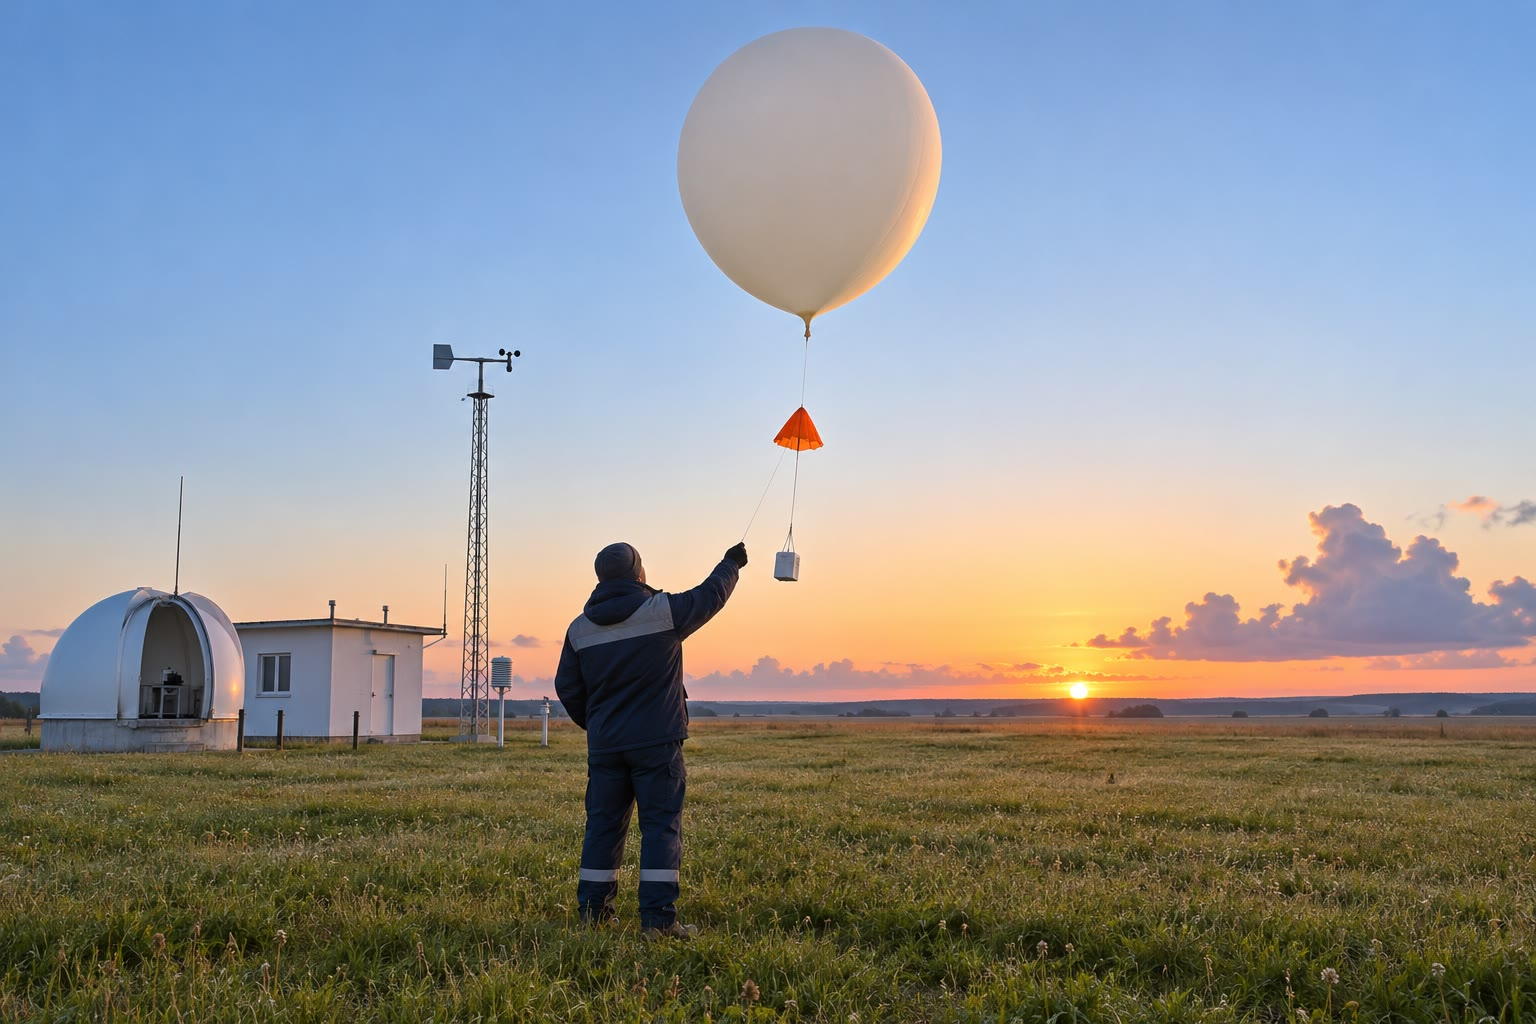
\includegraphics[width=\linewidth]{images/book4/ai/b2-radiosonde-launch.jpg}

{\scriptsize A radiosonde released at dawn from a weather station (AI-generated
illustration).}
\end{minipage}
% ledger: nws:radiosonde, nws4:upperair
\end{inthefield}

\section*{Exercises}\label{sec:b2:atmospheric-thermodynamics:exercises}

Data for the exercises, unless stated otherwise: $e_s(T) = \qty{6.117}{hPa} \times
\exp[\qty{5419}{K} \times (1/\qty{273.16}{K} - 1/T)]$; $\varepsilon = 0.622$, $R_d =
\qty{287.0}{J.kg^{-1}.K^{-1}}$, $R_v = \qty{461.5}{J.kg^{-1}.K^{-1}}$, $c_p =
\qty{1004.5}{J.kg^{-1}.K^{-1}}$, $L = \qty{2.501e6}{J/kg}$, $g = \qty{9.81}{m.s^{-2}}$,
$\Gamma_d = \qty{9.8}{K/km}$.
% ledger: nist4:water-sat, iapws4:sublimation, const:R, earth:Mmol, nist4:water-mw, nasa:grc-gamma

\begin{exercise}[$\star$]\label{exo:b2:atmospheric-thermodynamics:1}
At \qty{850}{hPa} the temperature is \qty{10.0}{\celsius} and the dew point \qty{5.0}{\celsius}.
(a) Find the \omterm{def:b2:atmospheric-thermodynamics:moist-air}{vapour pressure} and the saturation \omterm{def:b2:atmospheric-thermodynamics:moist-air}{vapour pressure}. (b) Find the relative humidity.
(c) Find the \omterm{def:b2:atmospheric-thermodynamics:moist-air}{mixing ratio} and the \omterm{def:b2:atmospheric-thermodynamics:moist-air}{specific humidity}, in grams per kilogram.
\end{exercise}

\begin{exercise}[$\star$]\label{exo:b2:atmospheric-thermodynamics:2}
(a) By how many per cent per kelvin does $e_s$ rise at \qty{0}{\celsius}, \qty{20}{\celsius} and
\qty{30}{\celsius}? (b) Compute $e_s$ at \qty{20}{\celsius} and at \qty{25}{\celsius}, and their
ratio; compare with $1.063^5$. (c) The measured value at \qty{20}{\celsius} is
\qty{23.39}{hPa}. By how much does the formula err, and in which direction? Why?
\end{exercise}
% ledger: nist4:water-sat

\begin{exercise}[$\star$]\label{exo:b2:atmospheric-thermodynamics:3}
At noon the surface air is at \qty{30}{\celsius} with a dew point of \qty{14}{\celsius}. (a) At
what height above the ground do cumulus bases form? (b) What is the temperature of a parcel
there, by the dry adiabat? (c) What is its dew point there, with $\Gamma_{\text{dew}} =
\qty{1.8}{K/km}$? Comment. (d) Later the air warms to \qty{33}{\celsius}, the dew point
unchanged. Where are the cloud bases now?
\end{exercise}

\begin{exercise}[$\star$]\label{exo:b2:atmospheric-thermodynamics:4}
Read the skew-T diagram of the Norman sounding. (a) Up to which pressure is the air near the
ground saturated, or nearly so? (b) Where is the inversion, and how does it show? (c) Read the
LCL, the LFC and the EL of the surface parcel. (d) How do the dew point and the temperature
compare just above the inversion, and what does that say about this air?
\end{exercise}
% ledger: data:b4-sounding

\begin{exercise}[$\star\star$]\label{exo:b2:atmospheric-thermodynamics:5}
Tropical air at \qty{1000}{hPa} has $T = \qty{30.0}{\celsius}$ and $r = \qty{20}{g/kg}$. (a) Find
its \omterm{def:b2:atmospheric-thermodynamics:virtual}{virtual temperature} exactly and with the approximation $T(1 + 0.61\,r)$. (b) Find the densities
of this air and of dry air at the same temperature and pressure. (c) By how much would dry air
have to be warmed to be as light? (d) Why does this matter for convection over warm seas?
\end{exercise}

\begin{exercise}[$\star\star$]\label{exo:b2:atmospheric-thermodynamics:6}
Use \cref{prop:b2:atmospheric-thermodynamics:gamma-s} at \qty{1000}{hPa}, with $r_s$ from
\cref{prop:b2:atmospheric-thermodynamics:humidity}. (a) Compute $r_s$ and $\Gamma_s$ at
\qty{0}{\celsius}, \qty{20}{\celsius} and \qty{30}{\celsius}. (b) How much warmer than a dry
parcel is a saturated parcel at \qty{20}{\celsius} after rising \qty{1}{km}, if its lapse rate
stays the same? (c) Why does the difference shrink higher up?
\end{exercise}

\begin{exercise}[$\star\star$]\label{exo:b2:atmospheric-thermodynamics:7}
The Norman surface parcel ($p = \qty{971.1}{hPa}$, $T = \qty{19.0}{\celsius}$, $T_d =
\qty{18.5}{\celsius}$) has its LCL at \qty{18.35}{\celsius}. (a) Compute its \omterm{def:b2:atmospheric-thermodynamics:moist-air}{mixing ratio}, its
potential temperature and its \omterm{def:b2:atmospheric-thermodynamics:theta-e}{equivalent potential temperature}. (b) Lifted, it is at
\qty{-8.9}{\celsius} at \qty{500}{hPa}, saturated. Compute its $\theta$ and $\theta_e$ there.
(c) Which of the two is conserved?
\end{exercise}
% ledger: data:b4-sounding

\begin{exercise}[$\star\star$]\label{exo:b2:atmospheric-thermodynamics:8}
A parcel is warmer than its surroundings by \qty{4}{K} between \qty{700}{hPa}, its LFC, and
\qty{300}{hPa}, its EL; ignore the virtual-temperature correction. (a) Compute its CAPE. (b)
Compute $w_{\max}$. (c) Which class does the CAPE fall into? (d) On a skew-T diagram, what
shape has the positive area, and why is its area what was computed?
\end{exercise}
% ledger: hgx:cape

\begin{exercise}[$\star\star$]\label{exo:b2:atmospheric-thermodynamics:9}
Take $A = \qty{2.1}{nm}$ and ammonium sulfate, $\kappa = 0.61$. (a) Find the critical diameter
and \omterm{def:b2:atmospheric-thermodynamics:microphysics}{supersaturation} of a dry particle of \qty{80}{nm}. (b) What is the smallest dry particle
activated in air at \qty{0.3}{\percent} \omterm{def:b2:atmospheric-thermodynamics:microphysics}{supersaturation}? At \qty{0.1}{\percent}? (c) An updraft
raises the \omterm{def:b2:atmospheric-thermodynamics:microphysics}{supersaturation} from \qty{0.1}{\percent} to \qty{0.3}{\percent}: what happens to the
number of droplets, and to their size for the same liquid water?
\end{exercise}
% ledger: pk07:kappa, pk07:kohler

\begin{exercise}[$\star\star\star$]\label{exo:b2:atmospheric-thermodynamics:10}
The Norman surface parcel had a CIN of about \qty{-130}{J/kg} with the \omterm{def:b2:atmospheric-thermodynamics:virtual}{virtual temperature}.
(a) With what vertical speed would it have to leave the ground to reach its LFC by its own
momentum? (b) The inversion top is at \qty{889.1}{hPa} and \qty{20.5}{\celsius}. To what
temperature must the surface air at \qty{971.1}{hPa} warm for a parcel lifted dry
adiabatically to be no colder than the inversion top? (c) If its dew point stayed at
\qty{18.5}{\celsius}, where would its cloud base be? (d) Name two ways in which the atmosphere
removes such a lid without the sun.
\end{exercise}
% ledger: data:b4-sounding, nws4:cin

\begin{exercise}[$\star\star\star$]\label{exo:b2:atmospheric-thermodynamics:11}
(a) Show from \cref{prop:b2:atmospheric-thermodynamics:gamma-s} that $\Gamma_s \to \Gamma_d$
as $r_s \to 0$. (b) Show that when $Lr_s/(R_dT) \gg 1$, $\Gamma_s \to gR_vT/(LR_d)$, and
evaluate it at \qty{303}{K}. (c) Compare with $\Gamma_{\text{dew}}$ of
\cref{prop:b2:atmospheric-thermodynamics:lcl} when $T_d = T$, and explain why the two limits
coincide. (d) Is the limit of (b) reached in the atmosphere? Use the value $\Gamma_s =
\qty{3.4}{K/km}$ at \qty{30}{\celsius} and \qty{1000}{hPa}.
\end{exercise}

\begin{exercise}[$\star\star\star$]\label{exo:b2:atmospheric-thermodynamics:12}
Over supercooled water and over ice the saturation \omterm{def:b2:atmospheric-thermodynamics:moist-air}{vapour pressures} are 2.868 and
\qty{2.599}{hPa} at \qty{-10}{\celsius}, 1.257 and \qty{1.032}{hPa} at \qty{-20}{\celsius}.
(a) Find the \omterm{def:b2:atmospheric-thermodynamics:microphysics}{supersaturation} over ice of air saturated over water at both temperatures. (b)
Compare with the \omterm{def:b2:atmospheric-thermodynamics:microphysics}{supersaturations} at which droplets activate. (c) Explain why a cloud of
supercooled droplets that receives a few ice crystals turns to ice. (d) Why is the effect
weaker near \qty{0}{\celsius}?
\end{exercise}
% ledger: iapws4:sublimation, su26:svp, nws4:ccn-bergeron

\begin{problem}[{Weekend problem --- Reading the morning sounding}]\label{pb:b2:atmospheric-thermodynamics:1}
The table gives the 12 UTC sounding of Norman, Oklahoma, on 16 April 2026, at the levels used
here: pressure, height above sea level, temperature, dew point, and the temperature of the
surface parcel lifted as in \cref{met:b2:atmospheric-thermodynamics:lift}, computed by
integrating \cref{prop:b2:atmospheric-thermodynamics:gamma-s} in small steps. The sounding
reports the tropopause at \qty{235.3}{hPa} and \qty{10954}{m}. Use the data of the exercises and
the temperatures (not the \omterm{def:b2:atmospheric-thermodynamics:virtual}{virtual temperatures}) unless told otherwise.

\begin{center}
\small
\begin{tabular}{rrrrr}
\hline
$p$ (\unit{hPa}) & $z$ (\unit{m}) & $T$ (\unit{\celsius}) & $T_d$ (\unit{\celsius}) &
$T_{\text{parcel}}$ (\unit{\celsius}) \\
\hline
971.1 & 345 & 19.0 & 18.5 & 19.0 \\
925.0 & 763 & 17.3 & 17.3 & 16.9 \\
907.7 & 924 & 16.4 & 16.4 & 16.2 \\
889.1 & 1102 & 20.5 & 9.5 & 15.4 \\
850.0 & 1489 & 18.6 & $-1.8$ & 13.7 \\
700.0 & 3110 & 4.5 & $-12.2$ & 6.1 \\
500.0 & 5725 & $-18.4$ & $-36.6$ & $-8.9$ \\
400.0 & 7357 & $-30.4$ & $-55.6$ & $-20.4$ \\
300.0 & 9349 & $-42.7$ & $-66.3$ & $-37.1$ \\
250.0 & 10560 & $-49.8$ & $-69.8$ & $-48.3$ \\
200.0 & 12006 & $-52.3$ & $-78.3$ & $-61.8$ \\
\hline
\end{tabular}
\end{center}

\medskip\noindent\textbf{Part I --- The air near the ground.}
\begin{enumerate}
  \item Find the \omterm{def:b2:atmospheric-thermodynamics:moist-air}{vapour pressure} of the surface air, to one decimal.
  \item Find its \omterm{def:b2:atmospheric-thermodynamics:moist-air}{mixing ratio}, to one decimal.
  \item Find its \omterm{def:b2:atmospheric-thermodynamics:moist-air}{specific humidity}.
  \item Find its relative humidity.
  \item By how much does its \omterm{def:b2:atmospheric-thermodynamics:virtual}{virtual temperature} exceed its temperature?
  \item Find the height of its LCL above the ground with the \qty{125}{m} rule, and the pressure
        there (take a mean \omterm{def:b2:atmospheric-thermodynamics:virtual}{virtual temperature} of \qty{294.7}{K} for the layer).
  \item Find its potential temperature.
\end{enumerate}

\medskip\noindent\textbf{Part II --- The lid and the layers above.}
\begin{enumerate}[resume]
  \item At \qty{925}{hPa}, is the parcel warmer or colder than its surroundings, and by how much?
  \item Find the lapse rate between 907.7 and \qty{889.1}{hPa}. What kind of layer is this?
  \item By how much is the parcel colder than its surroundings at \qty{889.1}{hPa}?
  \item Find the relative humidity at \qty{850}{hPa}. Where could such air have come from?
  \item Find the mean lapse rate between 850 and \qty{500}{hPa} and classify the layer.
  \item Find the lifted index and its class.
\end{enumerate}

\medskip\noindent\textbf{Part III --- The energy.}
\begin{enumerate}[resume]
  \item Compute the excess $\Delta T = T_{\text{parcel}} - T$ at each level of the table.
  \item Find the LFC by interpolating $\Delta T$ linearly in $\ln p$, to the nearest hectopascal,
        and its height by interpolating $z$ the same way.
  \item Find the EL and its height in the same way. Compare with the tropopause.
  \item Compute the CAPE by the trapezium rule in $\ln p$, from the LFC to the EL through the
        levels of the table.
  \item Which class does it fall into?
  \item Compute the CIN in the same way, from the ground to the LFC.
  \item A computation on a grid of \qty{1}{hPa} gives a CAPE of \qty{2100}{J/kg} with the
        temperatures and \qty{2230}{J/kg} with the \omterm{def:b2:atmospheric-thermodynamics:virtual}{virtual temperatures}. Why do the three values
        differ?
\end{enumerate}

\medskip\noindent\textbf{Part IV --- The storm the air could feed.}
\begin{enumerate}[resume]
  \item What vertical speed does parcel theory give with the CAPE of question 17?
  \item At half that speed throughout, how long would the air take to rise from the LFC to the EL?
  \item Name two effects that make a real updraft slower.
  \item To sum up: what updraft speed does parcel theory predict for a storm fed by this
        morning's surface air?
\end{enumerate}
\end{problem}
% ledger: data:b4-sounding, hgx:cape, nws4:lifted-index, nws4:cape
